\documentclass{article}
\usepackage[preprint]{icml2026}
\usepackage{xeCJK}
\xeCJKsetup{CJKspace=true}
\setmainfont[BoldFont=texgyretermes-bold.otf,ItalicFont=texgyretermes-italic.otf,BoldItalicFont=texgyretermes-bolditalic.otf]{texgyretermes-regular.otf}
\setCJKmainfont[Path=fonts/,AutoFakeBold=2]{NotoSansCJKkr-Regular.otf}
\setCJKsansfont[Path=fonts/,AutoFakeBold=2]{NotoSansCJKkr-Regular.otf}
\usepackage{amsmath,amssymb,booktabs,graphicx,algorithm,algorithmic,tabularx}
\usepackage{hyperref}
\usepackage{xurl}
\icmltitlerunning{PCA + R5: Consecutive Residual Confirmation}
\newcommand{\ind}{\mathbf{1}}
\begin{document}
\twocolumn[
\icmltitle{기존 PCA 경보를 보존하는 예측잔차 연속 확인:\\재사용 유압펌프 자료에서의 미탐 감소와 오경보 대조 분석}
\begin{icmlauthorlist}
\icmlauthor{익명 연구 초안}{anon}
\end{icmlauthorlist}
\icmlaffiliation{anon}{저자·소속·지원기관 미확정}
\icmlcorrespondingauthor{Anonymous}{Not specified}
\makeatletter\gdef\icmlcorrespondingauthor@text{not specified (anonymous draft)}\makeatother
\icmlkeywords{이상탐지, PCA, 예측잔차, 연속 확인, 데이터 재사용, 재현성}
\vskip 0.15in
]
\makeatletter\gdef\icmlcorrespondingauthor@text{not specified (anonymous draft)}\makeatother
\printAffiliationsAndNotice{한국어 연구용 확장 원고. 기존 프로젝트의 2단 연구 원고·Noto 한글 서체·표와 캡션 형식을 계승했다. 공식 ICML 제출본·채택 논문이 아니며 저자 정보는 익명 상태다.}
\begin{abstract}
기존 PCA 검출기의 경보를 보존하면서 예측잔차 보조 경보를 추가하면, 관측된 오경보 증가를 억제하면서 미탐을 줄일 수 있는가? 본 연구는 정상 자료로 적합한 고정 PCA와 두 과거 관측을 입력으로 사용하는 ridge 예측기를 결합하고, 현재와 직전 잔차 점수가 모두 임계값을 초과할 때만 보조 경보를 허용하는 ``PCA + R5 예측잔차 보조 경보(G1)''를 조사한다. 이미 공개된 과거 평가 H의 정상 3,990행·이상 357행에서 미탐은 28행에서 13행으로 감소하고 오경보는 1행으로 유지되었다. F1은 0.957787에서 0.980057, F2는 0.935722에서 0.970107로 변했다. 같은 임계값에서 연속 확인을 없애면 미탐 10행·오경보 4행으로 바뀌어 확인 규칙의 손익이 드러났다. 추가 탐지 15행은 이미 탐지하던 세 관측 구간의 탐지 범위 확대이며 새 사건 발견은 0개다. 재사용 후반 V는 양쪽 오류가 없어 성능 유지에는 부합하지만 미탐 감소 재현은 판단할 수 없다. 모든 고유 관측의 기존 사용, 정상·이상 수집일 차이, 실제 고장 시작과 독립 신규 자료의 부재를 공개한다. 본 결과는 재현 가능한 제한적 사례 분석이며 현장 일반화·통계적 유의성·범용 알고리즘의 신규성을 입증하지 않는다.
\end{abstract}

\section{서론}
유압펌프 이상탐지의 운영 목표는 정상 관측을 많이 맞혀 전체 정확도를 높이는 것만으로 설명되지 않는다. 이상 관측의 미탐을 줄이는 동시에 정상적인 센서 변화에 대한 오경보를 관리해야 한다. 특히 정상 관측이 다수인 자료에서는 높은 Accuracy가 실제로 놓친 이상을 가릴 수 있다. 반대로 Recall만 올리면 정상 관측에 과도한 경보를 낼 수 있다. 따라서 같은 관측 행에서 TP, FN, FP, TN을 함께 보고, 미탐 감소가 추가 오경보를 대가로 얻어졌는지 구별해야 한다.

또 하나의 문제는 평가 단위다. 연속된 이상 관측 15행을 더 탐지했다는 사실은 서로 독립인 고장 15건을 추가로 발견했다는 뜻이 아니다. 이미 일부를 탐지한 관측 구간에서 경보 범위만 넓어졌을 수도 있다. 실제 고장 시작 이전의 정상 구간이 없다면 첫 기록 이후 경보까지의 시간을 고장 예측 선행시간으로 바꿔 해석할 수도 없다. 본 연구는 이 구분을 결과 해석의 중심에 둔다.

대상은 이전에 선정된 이동 통계 PCA 운영 모델 B0다. 이를 다른 PCA나 Forest 모델로 교체하지 않고, 기존 경보를 OR 연산으로 보존한다. 추가 경로 R5는 두 시점의 과거 센서로 현재 센서를 예측하는 정상 전용 ridge 회귀와 예측잔차 공분산 거리다. ``R5''는 선행 실험의 점수 식별자이며 5차 예측기라는 뜻이 아니다. G1은 R5 잔차가 현재와 직전 관측에서 모두 임계값을 초과한 경우에만 경보를 추가한다.

기여는 고정 운영 체계의 명세, 동일 행 대조 실험, 실행·데이터 사용 이력의 추적에 있다. PCA 잔차, 예측잔차, OR 결합, 연속 확인 각각의 발명을 주장하지 않는다. 선행 실험에서 이미 여러 번 사용한 자료라는 사실 때문에, 보존된 결과를 엄밀하게 재현하는 일과 새로운 자료에서 성능을 검증하는 일은 구분되어야 한다. 검출기 자체는 정상 자료로 학습하지만 후보 선택에는 개발 이상 라벨을 사용했으므로 전체 과정을 완전 비지도라고 부르지 않는다.

\section{관련 연구와 본 연구의 위치}
\subsection{PCA 잔차와 시간적 예측잔차}
\citet{jackson1979}은 일부 주성분으로 복원되지 않는 잔차에 대한 감시 절차를 다룬다. 본 연구의 Q는 표준화된 특징과 그 PCA 복원값 사이 제곱거리다. 원문에서 다루는 분포·공분산 가정을 현재 자료가 만족한다고 가정하지 않으며, 이론적 관리한계 대신 정상 calibration의 경험 분위수를 사용한다. 이 차이는 명목 임계값과 실제 운영 오경보율을 혼동하지 않기 위해 필요하다.

시간 상관구조에 대한 관점은 \citet{jiang2017}의 CVA 기반 연구와 연결된다. 그러나 본 연구의 두 지연 ridge 예측잔차는 해당 논문의 Rs/Rr 알고리즘이나 500관측치 창을 재현한 것이 아니다. 해당 문헌의 모의 시스템 결과를 유압펌프 성능으로 전이하지 않는다. 현재 R5는 미래 관측 벡터를 입력하지 않고, 현재 관측이 도착한 후 예측 오차를 계산한다.

잔차 거리의 공분산에는 \citet{ledoit2004}의 수축 추정 개념을 사용한다. 공분산 수축의 추정 성질이 곧바로 F1이나 F2의 향상을 보장하는 것은 아니다. 정상 학습의 중첩 시계열 예제는 독립 동일분포 관측과 다르며, 해당 이론을 이용해 본 자료에서 유의성을 주장하지 않는다.

\subsection{연속 확인과 평가 단위}
\citet{nist}의 관리도 설명은 연속 패턴 규칙과 민감도·오경보의 절충을 다룬다. G1의 정확한 두 관측 연속 초과, 두 calibration 분위수, OR 보존은 이 프로젝트의 설계다. 기존 WECO 규칙의 재현이나 최적 규칙의 증명으로 표현하지 않는다. 인접 잔차가 의존하므로 단일 초과 확률이 $p$일 때 연속 초과 확률을 단순히 $p^2$라고 계산하지 않는다.

\citet{tatbul2018}은 시계열에서 구간을 고려한 평가의 필요성을 보여준다. 본 연구는 행 단위 판정을 유지한 채 관측 구간 탐지 여부와 범위 확장을 별도로 제시한다. 한 행을 탐지했다고 구간 전체를 정탐으로 바꾸는 point adjustment는 하지 않는다. \citet{saito2015}의 불균형 평가 관점에 따라 PR 지표를 보조적으로 보고하고, \citet{chicco2020}과 연결해 MCC도 부록에 계산한다. 다만 같은 혼동행렬에서 나온 여러 지표는 서로 독립된 실험 증거가 아니다.

\subsection{반복 선택과 시간 검증}
\citet{cawley2010}은 모델 선택 기준 자체가 과적합될 가능성과 평가 편향을 논의한다. 이 문헌은 반복 개발 위험을 설명하지만 본 모델의 과적합 크기가 이미 측정됐다는 근거는 아니다. \citet{bergmeir2018}은 자기회귀 시계열 교차검증의 적용 조건을 다루며 모든 시계열의 무작위 교차검증을 금지하는 논문이 아니다. 본 연구의 핵심 한계는 동일 기록의 반복 사용과 새 독립 자료의 부재다. 이미 사용한 구간에 새 이름을 붙이는 것으로 그 한계가 해소되지 않는다.

\section{자료 진단과 역할 복원}
\subsection{원본, 관측, 라벨}
프로젝트에서 제공한 소성가공 예지보전 자료의 정상 CSV는 20,000행, 이상 CSV는 600행이다. 정상 파일의 11566번째 데이터 행은 첫 열 번호만 다르고 TimeStamp·센서·Equipment\_state가 11565행과 같아 분석에서 제외했다. 원본 파일은 수정하지 않았으며 CSV 헤더를 포함한 줄 번호는 각각 11567, 11566이다. 분석 고유 관측은 정상 19,999행·이상 600행으로 총 20,599행이다. 중복도 이미 사용한 관측과 같으므로 미사용 시험 자료가 아니다.

모델 센서는 AI0\_Vibration, AI1\_Vibration, AI2\_Current다. 각 물리 단위, AI0/AI1의 상부·하부 대응, 장비 식별자와 운전 부하는 미확인이다. Equipment\_state는 정상 0·이상 1의 정답이며 센서 입력에 포함하지 않는다. 빈 이름의 첫 열, 파일명, 날짜, 원행 번호와 burst ID도 수치 입력에서 제외한다. 시각과 구간 ID는 인과적 입력 범위와 상태 초기화, 결과 추적에 사용한다. 음의 전류와 큰 센서값은 임의 삭제하거나 절댓값으로 변환하지 않는다.

정상 수집일은 2022-07-12, 이상 수집일은 2022-07-17이다. 이 날짜 차이는 확인되지만 날짜별 운전조건의 구체적인 차이는 기록이 없다. 라벨과 날짜가 함께 바뀌므로 고장 효과와 취득·운전조건 효과를 분리하기 어렵다. 압력, 불량, 비가동, 정비 이력과 실제 고장 시작도 없다. 이 자료로 해당 결과를 직접 예측하거나 감소시켰다고 주장하지 않는다.

\subsection{관측 공백과 고정 분할}
중복 제거 후 인접 시간 차이가 0.5초를 초과하면 새로운 관측 연속 구간을 만든다. 정상은 599개, 이상은 21개 구간이다. 0.5초 초과 공백은 각각 598곳·20곳, 최대 공백은 16.643초·8.572초다. 중앙 관측 간격은 0.1초지만 20행의 실제 경과시간은 일정하지 않다. 큰 공백을 보간하지 않으며 FFT 특징도 사용하지 않는다. 이 sampling 정보만으로 앨리어싱을 확정하거나 PCA가 그 영향을 제거한다고 쓰지 않는다.

\begin{table}[t]\centering\small
\caption{원래 시간순 역할과 G1에서의 역할. S는 S1과 S2의 합집합이다. 두 클래스의 시각 순서를 각각 보존하며 같은 시각의 관측처럼 취급하지 않는다.}\label{tab:data}
\begin{tabular}{lrrl}\toprule
역할 & 정상 & 이상 & 현재 용도\\\midrule
T &12012&0&정상 학습\\
C &2011&132&정상 임계값 산출\\
S1 &639&18&후보 선택\\
S2 &616&3&후보 선택\\
V &731&90&재사용 유지 점검\\
H &3990&357&노출된 과거 평가\\\bottomrule
\end{tabular}
\end{table}

원래 분할은 파일 내 시간순으로, 관측 구간을 쪼개지 않도록 고정했다. T 내부에는 기존 실험의 fit 10,198행과 early\_stop 1,814행 역할이 남아 있다. PCA는 early stopping을 하지 않고 둘 다 학습하지만 입력 창은 그 경계에서 초기화한다. C의 이상 132행은 과거 sigmoid 보정 등에서 사용됐으나 현재 G1의 정상 임계값 산출에는 사용하지 않는다.

S1/S2/V는 원래 selection 2,097행을 재구분한 것이다. 보고용 경계라는 이유로 실제 연속 입력 상태를 새로 초기화하지 않는다. 따라서 V 초반 B0 창은 같은 원래 selection 안의 이전 S 관측을 문맥으로 포함할 수 있다. 이는 원래 train/calibration/test 분할을 넘는 fit이나 미래 참조와 다르지만, V가 문맥까지 완전히 독립이라는 해석을 막는다. 입력 창·warm-up 이력을 행별 감사표에 보존했다.

\section{방법: 고정된 PCA와 R5의 결합}
\subsection{기존 PCA B0}
B0의 주 경로 P1은 같은 원래 분할·파일 내에서 현재를 포함한 과거 20행을 사용한다. 시간 공백을 가로지를 수 있는 이동 통계다. 센서별 평균, 표준편차($ddof=0$), RMS, 최솟값, 최댓값을 계산해 15개 특징을 만든다. 특징 순서는 통계 종류가 먼저이고 그 안에서 AI0, AI1, AI2 순이다. 윈도 내부의 모든 순서를 학습하는 모델은 아니다.

창이 부족한 첫 19행은 단일 관측의 세 센서를 쓰는 P0로 보완한다. 두 경로는 각각 정상 T에서 적합한 StandardScaler와 full SVD, whiten=False, 주성분 2개의 PCA를 사용한다. 정상 학습 입력은 P1 완전 창 11,974개와 P0 행 12,012개다. 실제 유효 rank는 15와 3이며 선택 모델에서 제거된 상수 특징은 없다. 모든 차원을 복원해 잔차가 0이 되는 모델을 사용하지 않는다.

표준화 특징을 $z_t$, PCA 중심을 $\mu$, 주성분 열벡터 행렬을 $P$라 하면 Q는
\begin{equation}
Q_t=\|(z_t-\mu)-PP^\top(z_t-\mu)\|_2^2
\end{equation}
다. 경로마다 정상 C 점수의 95백분위수로 나누어 혼합한다. P1의 참조값은 14.9874861938813, P0는 2.649158116699839다. 경로 $w(t)$에 대해 $q_t=Q_t/c_{w(t)}$로 놓으면, 원 B0 경보는 $b_t=\ind[q_t>\eta]$이며 $\eta=1.3078792257682357$이다. 정상 C의 전체 운영 점수에서 목표 FPR 1\%에 해당하는 higher 분위수로 계산했다. 동점은 비경보다. 이 비율은 고장 확률이 아니며 B0 경보 자체에는 후처리가 없다.

\subsection{R5 예측기와 예측잔차 점수}
R5는 원 센서 벡터를 별도 정상 T StandardScaler로 표준화한 $v_t\in\mathbb R^3$를 쓴다. 동일 관측 연속 구간의 직전 두 관측을 결합해 $u_t=[v_{t-1}^\top,v_{t-2}^\top]^\top$로 두고 현재 $v_t$를 예측한다. 중앙화한 정상 학습 행렬을 $U_c,Z_c$, 유효 예제 수를 $n$이라 하면
\begin{align}
W&=(U_c^\top U_c/n+\lambda I)^{-1}U_c^\top Z_c/n,\\
\widehat v_t^\top&=(u_t-\bar u)^\top W+\bar v^\top,\\
\lambda&=10^{-3}\operatorname{tr}(U_c^\top U_c/n)/6
\end{align}
으로 계산한다. 절편은 정규화하지 않는다. 실제 학습 예제는 11,296개, $\lambda$는 0.0010006424934215698이다. ``2시점''은 입력 지연의 수이며 두 시점 뒤를 예측한다는 뜻이 아니다.

잔차 $e_t=v_t-\widehat v_t$에 대해 정상 학습 잔차의 평균 $\bar e$와 Ledoit--Wolf 공분산 $\Sigma$를 사용한다. 점수는
\begin{equation}
s_t=(e_t-\bar e)^\top(\Sigma+\epsilon I)^{-1}(e_t-\bar e),
\end{equation}
이며 $\epsilon=10^{-10}\operatorname{tr}(\Sigma)/3$다. 구현은 역행렬의 직접 계산 대신 Cholesky 선형해법을 사용한다. 새 scaler, 회귀 계수와 잔차 공분산은 모두 정상 T에만 적합한다.

정상 C 2,011행 중 1,889행에서 잔차를 계산할 수 있고 122행은 구간 시작 등의 이유로 unavailable이다. 선정 임계값은 이 유효 점수의 99.9백분위수, $\theta=17.54312199063481$이다. NumPy higher 계산의 정렬된 0기반 인덱스는 1887이며 동점 1개, strict 초과 1개다. 보정 분포의 해상도는 $1/1889$다. 유효 점수에서 분위수를 계산했다는 사실과 전체 행 운영 분모를 구별하며, 실제 미래 FPR가 0.1\%가 된다고 보장하지 않는다.

\subsection{현재·직전 초과와 상태 초기화}
$h_t=\ind[s_t>\theta]$로 정의하고 점수가 unavailable이거나 경계 이전의 상태이면 0으로 놓는다. 최종 G1 경보는
\begin{equation}\label{eq:gate}
g_t=b_t\lor(h_t\land h_{t-1})
\end{equation}
이다. 직전 관측은 같은 연속 구간에서 바로 앞에 수신한 관측이며 보간된 고정시간 격자가 아니다. 두 과거 관측이 필요한 R5와 직전 잔차 확인을 합하면 보조 경보의 원자료 의존 범위는 최대 $t,t-1,t-2,t-3$ 네 행이다.

파일·원래 분할·T 내부 역할 경계에서는 두 경로 상태를 초기화한다. 0.5초 초과 공백에서는 R5 지연과 확인 상태를 초기화하지만 P1 특징 창은 유지한다. 처음 두 관측은 R5 점수가 없고 첫 보조 G1 경보는 빠르면 네 번째 관측부터 가능하다. 현재 예측 오차에는 실제 현재 센서값이 필요하므로 경보 가능 시각은 현재 관측 도착 후다. 예측값을 미리 계산할 수 있어도 경보를 이전 관측으로 소급하지 않는다. 계산 지연은 타임스탬프 기반 가용 시각과 별개다.

같은 행에서 $b_t\le g_t$이므로 기존 TP는 감소하지 않고 FN은 증가하지 않는다. 동시에 FP도 감소할 수 없다. 이 구조만으로 FP가 유지된다는 결론은 나오지 않는다. 같은 임계값의 단일 초과 $h_t$에 비해 $h_t\land h_{t-1}$의 집합은 작으므로 연속 확인은 짧은 이상도 놓칠 수 있다. 이는 단순 집합 포함 관계이며 새로운 범용 학습 정리로 제시하지 않는다.

\begin{figure*}[t]\centering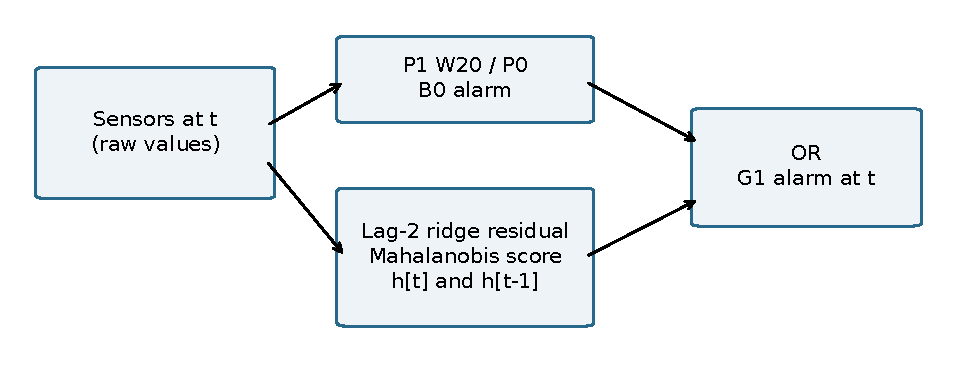
\includegraphics[width=.95\textwidth]{figures/flow.pdf}
\caption{고정 B0 경보와 R5 연속 초과의 OR 결합. B0 경보 자체를 지우거나 지연시키지 않는다. 관측 공백에서 특징 창과 경보 상태의 초기화 정책은 서로 다르다. 도식의 모든 예측 입력은 현재까지의 관측이다.}\label{fig:flow}
\end{figure*}

\section{평가 설계와 변경 이력}
\subsection{엄격 개선과 유지의 구별}
선택 합산 S에서는 FN의 엄격 감소, F2의 엄격 증가, F1의 비감소를 요구했다. S1/S2와 후반 V에서는 FN 비증가, F2/F1 비감소라는 유지 조건을 사용했다. 모든 필수 평가 블록에는
\begin{equation}
\Delta FP\le\lfloor0.001N_0\rfloor,\qquad
FP\le\lfloor0.01N_0\rfloor
\end{equation}
를 적용했다. $N_0$는 해당 블록의 정상 행 수다. S2의 정상 616행에서는 추가 FP를 한 개도 허용하지 않는다. 작은 표본이라는 이유로 최소 한 개를 허용하지 않았고, 비율 0.001은 0.1\%p 증가다. 정수 예산은 정확한 floor, 지표 비교 허용오차는 $10^{-12}$다.

V에서 FN $0\to0$은 유지 통과이며 감소 재현 여부는 not\_assessable이다. F2 $1\to1$도 유지 통과다. 정상만 있는 블록은 FP/FPR만 평가한다. F1과 F2는 각각 $2TP/(2TP+FN+FP)$, $5TP/(5TP+4FN+FP)$로 계산한다. F2의 가중치 네 배를 실제 고장 비용의 네 배로 해석하지 않는다. 이 기준은 잠정 프로젝트 정책이며 대회 공식 평가 기준이 아니다.

\subsection{선행 실패와 여섯 구성}
선행 문헌 기반 실험은 6개 보조 점수와 3개 추가 calibration FP 예산의 18개 구성을 실행했지만 선정 후보가 없었다. 그때 V 기준선 FN이 0이고 F2가 1인데도 strict 개선을 요구한 정책은 후속 실험에서 유지 조건으로 분리했다. 이 변경은 평가 규칙 수정이지 모델 점수 개선이 아니다.

기존 R5\_A0/A1은 합산 S에서 FN $3\to1$을 보였지만 S2에서 FN $0\to0$, FP $6\to7$이었다. FPR은 0.974026\%에서 1.136364\%로 증가했고 F1/F2도 하락했다. 그러므로 V 정책 수정은 이 S2 탈락을 취소하지 않는다. 해당 선행 R5의 V 성능은 당시 미평가였으며, 나중의 고정 대조 결과와 혼동하지 않는다.

후속 개발은 G0(현재 초과), G1(현재·직전 초과), G2(현재 초과와 직전 둘 중 하나 초과)를 정상 C 분위수 0.995, 0.999에서 비교했다. 여섯 구성의 점수를 계산한 뒤 중복 판정을 제외했다. G0의 높은 분위수는 이전 R5\_A1과 같은 구성이다. G2는 각 분위수에서 G1과 C/S 이진 판정이 같았지만 규칙과 연속 점수까지 보편적으로 같지는 않다. 선정은 G1, 0.999였다. 적격 후보의 합산 F2, 적은 FP, 단순한 규칙 순서로 고정했으며 이후 대조군의 H 점수로 교체하지 않았다.

\subsection{사전 고정과 반복 노출의 범위}
로컬 기록에서 선정 설정 생성은 2026-10-04 12:53:34 UTC, 뒤따른 평가 명령은 12:53:55 UTC다. 이는 해당 회차의 순서를 뒷받침하지만 현재 해시만으로 과거 사전 고정을 증명하는 것은 아니고 외부 공증 시각도 아니다. 더구나 같은 S/V/H는 이미 최소 네 번의 선행 개발 회차에서 사용됐다. 사용자 요청 기록에는 기존 S2 오경보 결과를 보고 확인 규칙을 시험하라고 방향을 바꾼 근거가 남아 있다. 개발 자료를 보고 다음 가설을 정한 것 자체를 부정행위로 보지 않되, 그 이력을 숨기지 않는다.

현재 G1 계열의 고유 구성은 개발 임계값 두 개와 사후의 이전 임계값 G1 대조군 한 개, 총 세 개다. 이와 학습 절차 수·전체 재실행·지표 재집계·구현 검사는 다른 단위다. 동일 자료 재실행은 독립 반복 실험이 아니다. 이번 원고에서 새 후보 탐색과 재선정은 수행하지 않았다.

\section{결과}
\subsection{동일 관측에서의 주 비교}
표~\ref{tab:main}은 저장된 행별 예측에서 공통 지표 코드로 다시 계산했다. S의 정상 1,255행·이상 21행에서 B0는 TP18/FN3/FP8/TN1247, G1은 TP19/FN2/FP8/TN1247이다. F1은 0.765957에서 0.791667, F2는 0.818182에서 0.855856으로 변했다. 개선은 S1에 집중되며 S2는 양쪽 TP3/FN0/FP6이다. S2의 정상 분모와 높은 FP 수준은 합산 결과만 제시하면 가려질 수 있다.

V의 정상 731행·이상 90행에서는 양쪽 TP90/FN0/FP0/TN731이다. 유지 조건은 통과하지만 줄일 기준선 FN이 없으므로 FN 감소의 재현은 판단 불가다. 이를 독립 자료에서 개선을 확인했다고 쓰지 않는다.

H에서 B0는 실제 이상 357행 중 329행 탐지·28행 미탐이며, G1은 344행 탐지·13행 미탐이다. 정상 3,990행 중 오경보는 각각 1행, 정상 1,000관측당 0.250627개다. Recall은 92.1569\%에서 96.3585\%, Precision은 99.6970\%에서 99.7101\%로 변했다. F1은 0.957787에서 0.980057, F2는 0.935722에서 0.970107로 증가했다. 기존 B0의 329개 탐지와 원 오경보 행이 모두 보존되었다. 이 결과는 노출된 과거 H에서 관찰한 개선이다.

\begin{table*}[t]\centering\small\caption{B0와 G1의 같은 원행 비교. 수는 관측 행이며 독립 고장 수가 아니다. FPR만 백분율이고 나머지 비율은 0--1이다. S는 S1/S2와 중첩한다.}\label{tab:main}\begin{tabular}{llrrrrrrrrrrr}
\toprule
Set & Model & $N_0$ & $N_1$ & TP & FN & FP & TN & Prec. & Recall & FPR(\%) & $F_1$ & $F_2$ \\
\midrule
S1 & B0 & 639 & 18 & 15 & 3 & 2 & 637 & 0.8824 & 0.8333 & 0.3130 & 0.8571 & 0.8427 \\
S1 & G1 & 639 & 18 & 16 & 2 & 2 & 637 & 0.8889 & 0.8889 & 0.3130 & 0.8889 & 0.8889 \\
S2 & B0 & 616 & 3 & 3 & 0 & 6 & 610 & 0.3333 & 1.0000 & 0.9740 & 0.5000 & 0.7143 \\
S2 & G1 & 616 & 3 & 3 & 0 & 6 & 610 & 0.3333 & 1.0000 & 0.9740 & 0.5000 & 0.7143 \\
S & B0 & 1255 & 21 & 18 & 3 & 8 & 1247 & 0.6923 & 0.8571 & 0.6375 & 0.7660 & 0.8182 \\
S & G1 & 1255 & 21 & 19 & 2 & 8 & 1247 & 0.7037 & 0.9048 & 0.6375 & 0.7917 & 0.8559 \\
V & B0 & 731 & 90 & 90 & 0 & 0 & 731 & 1.0000 & 1.0000 & 0.0000 & 1.0000 & 1.0000 \\
V & G1 & 731 & 90 & 90 & 0 & 0 & 731 & 1.0000 & 1.0000 & 0.0000 & 1.0000 & 1.0000 \\
H & B0 & 3990 & 357 & 329 & 28 & 1 & 3989 & 0.9970 & 0.9216 & 0.0251 & 0.9578 & 0.9357 \\
H & G1 & 3990 & 357 & 344 & 13 & 1 & 3989 & 0.9971 & 0.9636 & 0.0251 & 0.9801 & 0.9701 \\
\bottomrule
\end{tabular}
\end{table*}

\subsection{임계값과 연속 확인의 대조}
같은 선정 임계값에서 연속 확인을 없앤 G0는 H에서 FN10·FP4다. G1의 FN13·FP1과 비교하면 연속 확인은 오경보 세 행을 줄이면서 추가 탐지 가능했던 이상 세 행도 포기했다. 이 비교는 R5 점수와 임계값을 고정했으므로 확인 규칙의 효과로 해석할 수 있다.

이전 R5\_A0의 정확한 임계값 19.48692067098804에 G1을 적용하면 H에서 FN15·FP1이다. 같은 G1 구조에서 선정 임계값으로 바꾸면 FN이 두 행 더 줄고 FP는 같다. 확인 없는 이전 R5\_A0는 H의 FN11·FP3으로, 합산 H가 좋아 보여도 원래 S2 탈락을 번복하지 않는다. 표~\ref{tab:controls}와 그림~\ref{fig:tradeoff}의 대조는 사후 고정 분석이며 최고 점수 대조군을 새로운 선정 모델로 바꾸지 않았다.

\begin{table}[t]\centering\small\caption{정상 3,990·이상 357행의 H 대조. new는 선정 임계값, old는 정확한 이전 임계값이다.}\label{tab:controls}\begin{tabular}{lrrrr}
\toprule
Rule & FN & FP & $F_1$ & $F_2$ \\
\midrule
B0 & 28 & 1 & 0.957787 & 0.935722 \\
G1 & 13 & 1 & 0.980057 & 0.970107 \\
G0, new $\theta$ & 10 & 4 & 0.980226 & 0.975267 \\
G0, old $\theta$ & 11 & 3 & 0.980170 & 0.973551 \\
G1, old $\theta$ & 15 & 1 & 0.977143 & 0.965556 \\
\bottomrule
\end{tabular}
\end{table}
\begin{figure*}[t]\centering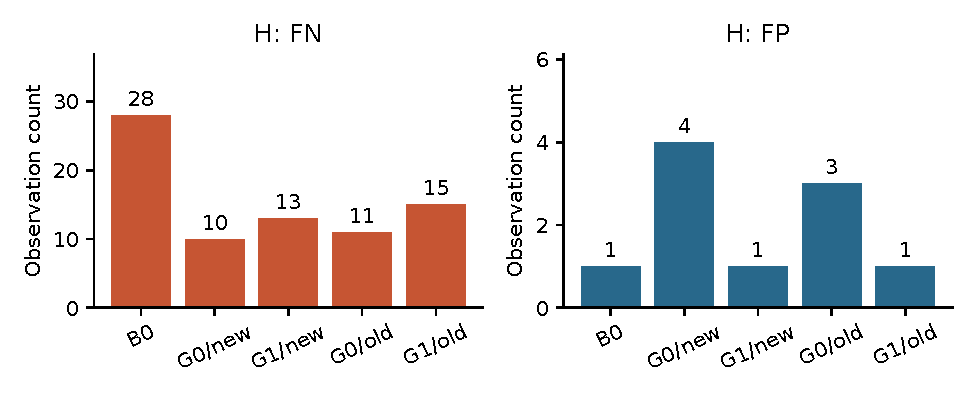
\includegraphics[width=.88\textwidth]{figures/fn_fp_H.pdf}\caption{고정 대조군의 H 미탐·오경보 수. 같은 임계값의 G0/G1은 확인 규칙을, old/new의 같은 규칙은 임계값 차이를 분리한다. 막대는 새로운 독립 자료의 성능이 아니다.}\label{fig:tradeoff}\end{figure*}

\subsection{사건, 탐지 범위와 시각}
기존 물리 사건 ID가 없어, 파일·원래 분할·0.5초 초과 공백 경계를 넘지 않는 연속 이상 라벨 구간을 임시 관측 사건으로 기술했다. H에는 13개가 있고 B0와 G1은 이미 모두 적어도 한 행을 탐지한다. 새로 발견한 전체 사건은 0개다. 추가 탐지 15행은 기존에 탐지하던 세 관측 구간에 분포한다. 따라서 미탐 행 감소와 새로운 사건 탐지 증가를 구별해야 한다.

가장 이른 추가 탐지 구간에서는 관측 시작부터 첫 경보까지의 실제 시각 차이가 0.4초에서 0.3초로 바뀌었다. 모든 H 이상 구간은 첫 기록부터 이상이므로 실제 시작은 왼쪽 절단되어 있다. 0.1초 변화는 실제 고장 발생 대비 탐지 지연이나 고장 전 예측 선행시간이 아니다. 미탐 사건의 지연을 0으로 대체하지 않으며 한 행 탐지로 전체 사건을 정탐 처리하지 않는다.

본문 수치와 연결되는 사례 그림은 시간순으로 가장 이른 추가 탐지 H 구간 전체를 표시하는 규칙으로 선정했다. 모델에는 들어가지 않는 미래 진단 문맥으로 판단을 소급하지 않는다. 모든 추가 탐지 구간과 모든 H 사건의 표를 부록에 제시해 유리한 사례 하나만으로 결론 내리지 않는다.

정상 H에서 B0와 G1의 오경보는 한 행이자 한 연속 에피소드다. 같은 구간 내 연속 정상 관측 사이 시간의 합은 387.2초다. 단순 관측 시간 정규화는 9.2975 에피소드/관측시간으로서의 시간당 값이지만 실제 가동시간 분모는 확인되지 않았다. 수집 공백을 정상 가동으로 더하지 않으며 이 값을 현장 시간당 오경보율로 보장하지 않는다.

\section{구현과 재현 검증}
원 모델 재로딩, batch와 한 행씩 입력하는 온라인 재생, 특징 순서, strict 동점, 상태 초기화와 미래값 변경 검사가 기존 기록에 남아 있다. 선택 당시와 고정 검증의 핵심 추론 코드 해시가 같다. 원래 온라인 보조 함수는 NaN을 받은 B0 점수를 비경보처럼 처리할 수 있어, 후속 외부 입력 검증기가 비유한 센서 입력 전체를 거부하도록 보완했다. 성능 자료에는 결측이 없으므로 원 결과의 판정은 변하지 않는다. 원 결과 생성 코드와 입력 검사 보완본의 역할을 구별해 함께 보존했다.

이번 패키지에서는 정상 원본으로부터 선택된 두 PCA 경로와 R5만 고정 설정대로 다시 적합하고, 정상 C만으로 참조값·임계값을 재산출했다. 재생성 모델은 별도 경로에 두고 선정 모델을 덮어쓰지 않았다. selection/H의 이진 경보는 완전히 일치했고 점수의 수치 비교에는 절대·상대 $10^{-9}$ 허용오차를 사용했다. R5 계수 비교는 $10^{-12}$로 확인했다. 저장 예측의 지표 재계산도 $10^{-12}$ 이내로 일치했다. 이것은 계산 재현이지 새 성능 표본이 아니다.

기본 실행은 과거 전체 탐색을 반복하지 않는다. 저장 모델 추론, 주요 표·그림 재생성, 고정 학습·calibration 재현, 새 CSV 입력 계약 검사, 원고 빌드와 SHA-256 검사를 각각 제공한다. 원본 경로는 출처에만 보존하고 실행 경로는 패키지 내부에서 결정한다. 별도 압축 해제 위치에서의 확인과 문서 빌드 기록을 verification에 둔다. 복구하지 못한 과거 인라인 실행과 전체 프로세스 이력은 원본이 있는 것처럼 재작성하지 않는다.

\section{논의와 한계}
관측된 결과는 연구 질문에 제한적으로 긍정적이다. 선정 G1은 기존 PCA 경보를 유지하면서 과거 H의 FN을 줄였고 FP는 늘리지 않았다. 그러나 이 결과는 OR 구조의 보장이 아니라 해당 표본에서의 결과다. 확인 없는 대조는 더 많은 이상을 탐지하면서 오경보도 늘렸으며, 확인 조건은 그 일부를 제거했다. 따라서 정확한 주장 단위는 PCA 단독 개선이 아닌 ``PCA + R5 예측잔차 보조 경보(G1)'' 운영 체계다.

첫째, 같은 S/V/H를 최소 네 회차의 선행 개발이 이미 사용했고 미사용 고유 관측이 없다. 새 이름의 블록, 모델 해시, 사전 고정 파일과 재실행은 이 노출을 없애지 않는다. 직접 기록은 결과 기반 후속 설계를 확인하지만 편향의 크기나 과적합 발생 자체를 정량적으로 확정하지는 못한다.

둘째, 클래스와 수집 날짜가 겹쳐 있고 실제 장비·운전 모드·부하·고장 유형의 정보가 없다. 다른 날짜·설비·부하에 일반화하거나 관측 센서 패턴을 고장 원인으로 확정할 근거가 없다. 단위도 확인되지 않아 센서값을 물리 임계치로 해석하지 않는다.

셋째, H의 추가 탐지는 세 관측 구간 안의 범위 확장이다. 실제 독립 고장 수와 시작 시각이 없으므로 새로운 사건 발견이나 고장 전 조기예측을 주장할 수 없다. V는 기준선부터 오류가 없어서 미탐 감소라는 방향의 증거가 추가되지 않는다. 20,599행을 독립 표본 수로 사용하는 유의성 검정이나 행 단위 bootstrap 신뢰구간은 수행하지 않았다.

넷째, 현재 대조는 선택된 B0에 대한 국소 변경을 설명한다. 다양한 최신 검출기에 대한 공정한 전체 비교나 방법의 범용 우월성을 입증하지 않는다. 재현 산출물의 양도 방법 신규성을 대신하지 않는다. 새 독립 수집 세션을 확보해 센서 의미·정상 운전·실제 고장 이력을 확인한 뒤, 고정 모델과 유지·개선 기준을 한 번 적용하는 것이 다음 검증에 필요하다.

\section{결론}
PCA + R5 예측잔차 보조 경보(G1)는 기존 경보를 보존하고 연속 예측잔차 초과만 추가하는 간단한 운영 결합이다. 노출된 과거 H에서 FN28에서 FN13으로 감소하고 FP1을 유지했지만, 그 의미는 이미 탐지한 관측 구간의 범위 확대다. 재사용 V에서는 성능 유지만 확인했고 독립 신규 자료 검증은 미실시다. 본 연구는 이 범위의 산술 결과·인과적 구현·반복 사용 이력을 재현 가능하게 제공하며, 계산 재현성을 현장 성능 입증으로 확대하지 않는다.

\section*{영향과 연구 상태}
잘못된 정상 판단은 정비를 늦출 수 있고 불필요한 경보는 생산 중단을 유발할 수 있다. 본 연구는 자동 제어 배포, 비가동 감소, 실제 고장 예방을 검증하지 않았다. 작성과 검토에 AI 보조를 사용했으며 별도 적대적 보고서는 저자 측 자체 검토다. 실제 외부 전문가 의견이나 ICML 심사 결과가 아니다. 저자·소속·지원·이해상충 사실은 미확정이며 임의로 없음이라고 선언하지 않는다. 데이터의 외부 재배포 권한은 별도 확인이 필요하고 이 패키지는 사용자 보관용으로 작성했다.
\bibliography{references}\bibliographystyle{icml2026}
\clearpage\appendix\onecolumn
\section{재현 명세와 온라인 의사코드}
한국어본은 기존 프로젝트의 ICML preprint 기반 연구용 확장 형식을 계승했으며 공식 익명 제출본이 아니다. 영문본은 ICML 2026 공식 기본 익명 양식을 사용하고 accepted 옵션을 쓰지 않는다. 두 문서는 같은 표·그림과 지표 생성 코드를 공유한다. 학습용 원본, 고정 분할, 선정 모델, 이전 등록, 실패 후보, 사용 이력과 실행 명령은 패키지의 독립 파일로 제공한다.

상수 특징 제거 기준은 정상 T 표준편차가 $10^{-12}\max(1,|\mathrm{mean}|)$보다 큰 특징을 유지하는 것이다. PCA rank는 고유값이 $\max(10^{-12},10^{-10}\lambda_1)$보다 큰 차원 수다. 선택 모델은 제거된 특징이 없고 $k=2$가 각각 rank보다 작다. 표준화 후 PCA 중심도 복원 잔차 식에 포함하며 inverse transform과 동일한 정의다. full SVD와 ridge를 seed만 바꿔 반복한 것을 안정성 증거로 사용하지 않았다.

\begin{algorithm}[h]\caption{완전한 센서 입력에서 선정 G1의 온라인 갱신}\begin{algorithmic}[1]
\REQUIRE 고정 PCA 두 경로, R5 scaler·회귀·공분산, $\eta$, $\theta$, 이전 상태
\STATE 현재 시각과 센서 벡터를 받는다. 외부 입력에 결측·무한대·시간 오류가 있으면 거부한다.
\IF{새 파일·원래 분할·해당 학습 역할 또는 실제 입력 세션}
\STATE P1 특징 창, R5 과거 입력, 직전 초과 상태를 초기화한다.
\ELSIF{직전 관측과 시각 차이가 0.5초 초과}
\STATE R5 과거 입력과 초과 상태만 초기화한다. P1 특징 창은 유지한다.
\ENDIF
\STATE 현재 센서를 특징 창에 넣고 W20 또는 P0로 $b_t$를 계산한다.
\STATE 같은 구간의 과거 두 관측이 있으면 현재 예측잔차로 $h_t=\ind[s_t>\theta]$를 계산하고, 없으면 0으로 둔다.
\STATE $g_t=b_t\lor(h_t\land h_{t-1})$를 현재 시각에 출력한다. 과거 행의 판정을 바꾸지 않는다.
\STATE 과거 입력과 현재 초과 상태를 저장한다. 보고용 S/V 경계에서는 상태를 유지한다.
\end{algorithmic}\end{algorithm}

실제 획득 세션 ID는 과거 자료에 없다. 신규 입력 인터페이스에서는 제공자가 확인한 session ID가 필요하며 임의 보고 블록을 세션으로 만들지 않는다. 단위·장비 호환성의 선언만으로 실제 호환성이 입증되는 것은 아니다. 결측을 보간하거나 판정 불가를 정상으로 대체하지 않으며 입력 검증을 통과한 경우에만 고정 모델을 적용한다.

\section{전체 지표 정의와 연속 점수}
Precision은 $TP/(TP+FP)$, Recall은 $TP/(TP+FN)$, FPR은 $FP/(FP+TN)$다. FNR은 $FN/(TP+FN)$, Specificity는 $TN/(TN+FP)$, NPV는 $TN/(TN+FN)$, Accuracy는 $(TP+TN)/N$이다. Balanced Accuracy는 Recall과 Specificity의 평균이고, MCC는 $(TP\cdot TN-FP\cdot FN)/\sqrt{(TP+FP)(TP+FN)(TN+FP)(TN+FN)}$이다. F0.5는 $1.25TP/(1.25TP+0.25FN+FP)$, FDR과 FOR는 각각 $FP/(TP+FP)$, $FN/(FN+TN)$다. 분모가 0이면 NA로 표시하며 이상이 없는 블록에는 이상 개선을 부여하지 않는다.

기존 코드에는 G1과 대응하는 연속 운영 점수 $a_t=\max(q_t/\eta,\min(s_t/\theta,s_{t-1}/\theta))$가 있다. unavailable과 초기화된 이전 비율은 0이며 $g_t=\ind[a_t>1]$다. AP는 Recall 증가량으로 Precision을 가중하고 PR-AUC는 사다리꼴 적분으로 별도 계산한다. R5 단독 AUC나 이진 경보의 AP를 G1 성능처럼 제시하지 않는다. 이 연속 점수의 cutoff 변경은 두 경로의 비율을 함께 바꾸는 분석으로, R5 임계값만 바꾼 대조와 다르다. S/V/H의 양성 비율이 달라 AP를 그대로 비교해 구간 순위를 정하지 않는다.

\begin{table}[!ht]\centering\caption{H 상세 지표. 정상 3,990·이상 357행의 같은 혼동행렬에서 산출했다.}\begin{tabular}{lrrrrrrrrr}
\toprule
Model & FNR & Spec. & NPV & Acc. & Bal.Acc. & MCC & $F_{0.5}$ & FDR & FOR \\
\midrule
B0 & 0.078431 & 0.999749 & 0.993030 & 0.993329 & 0.960659 & 0.955041 & 0.980918 & 0.003030 & 0.006970 \\
G1 & 0.036415 & 0.999749 & 0.996752 & 0.996779 & 0.981667 & 0.978475 & 0.990213 & 0.002899 & 0.003248 \\
\bottomrule
\end{tabular}
\end{table}
\begin{table}[!ht]\centering\caption{S 상세 지표. 정상 1,255·이상 21행.}\begin{tabular}{lrrrrrrrrr}
\toprule
Model & FNR & Spec. & NPV & Acc. & Bal.Acc. & MCC & $F_{0.5}$ & FDR & FOR \\
\midrule
B0 & 0.142857 & 0.993625 & 0.997600 & 0.991379 & 0.925384 & 0.766128 & 0.720000 & 0.307692 & 0.002400 \\
G1 & 0.095238 & 0.993625 & 0.998399 & 0.992163 & 0.949194 & 0.794204 & 0.736434 & 0.296296 & 0.001601 \\
\bottomrule
\end{tabular}
\end{table}
\begin{table}[!ht]\centering\caption{V 상세 지표. 정상 731·이상 90행. 완전 분류의 유지는 새로운 FN 감소 증거가 아니다.}\begin{tabular}{lrrrrrrrrr}
\toprule
Model & FNR & Spec. & NPV & Acc. & Bal.Acc. & MCC & $F_{0.5}$ & FDR & FOR \\
\midrule
B0 & 0.000000 & 1.000000 & 1.000000 & 1.000000 & 1.000000 & 1.000000 & 1.000000 & 0.000000 & 0.000000 \\
G1 & 0.000000 & 1.000000 & 1.000000 & 1.000000 & 1.000000 & 1.000000 & 1.000000 & 0.000000 & 0.000000 \\
\bottomrule
\end{tabular}
\end{table}
\begin{table}[!ht]\centering\caption{명시된 연속 운영 점수의 순위 지표. 구간별 양성 비율이 달라 구간 간 직접 순위 비교가 아니다.}\begin{tabular}{lrrrr}
\toprule
Set & Model & AP & PR-AUC & ROC-AUC \\
\midrule
S & B0 & 0.859801 & 0.859735 & 0.875052 \\
S & G1 & 0.906559 & 0.906516 & 0.917473 \\
V & B0 & 1.000000 & 1.000000 & 1.000000 \\
V & G1 & 1.000000 & 1.000000 & 1.000000 \\
H & B0 & 0.987098 & 0.987086 & 0.996203 \\
H & G1 & 0.995770 & 0.995766 & 0.999490 \\
\bottomrule
\end{tabular}
\end{table}
\begin{figure}[h]\centering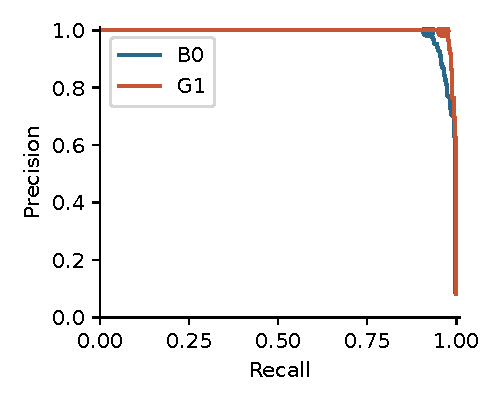
\includegraphics[width=.43\textwidth]{figures/pr_H.pdf}\caption{명시적으로 정의된 연속 운영 점수의 H PR 곡선. 점은 고정 운영점이다. 독립 일반화나 최적 임계값 재선정 결과가 아니다.}\end{figure}

\clearpage\section{관련 후보 전체와 탈락 사유}
\begin{table}[!ht]\centering\caption{후속 여섯 구성의 S 결과. 각 후보의 블록별 실패 문자열과 시간은 원 all\_trials.csv에 있다.}\begin{tabular}{lrrrrrr}
\toprule
Rule & $q$ & FN & FP & $F_1$ & $F_2$ & Decision \\
\midrule
G0 & 0.995 & 1 & 14 & 0.7273 & 0.8475 & ineligible \\
G0 & 0.999 & 1 & 9 & 0.8000 & 0.8850 & duplicate \\
G1 & 0.995 & 2 & 9 & 0.7755 & 0.8482 & ineligible \\
G1 & 0.999 & 2 & 8 & 0.7917 & 0.8559 & selected \\
G2 & 0.995 & 2 & 9 & 0.7755 & 0.8482 & duplicate \\
G2 & 0.999 & 2 & 8 & 0.7917 & 0.8559 & duplicate \\
\bottomrule
\end{tabular}
\end{table}
G0의 q=0.995는 S1 FP 예산 및 S2 FP/FPR/F1/F2를 위반한다. G0의 q=0.999는 이전 R5\_A1과 중복이며 S2에서 탈락한다. G1의 q=0.995 역시 S2에서 추가 FP가 한 행 생겨 FP/FPR/F1/F2 조건을 위반한다. G1의 q=0.999만 중복 제외 후 선정됐다. G2의 두 분위수는 해당 G1의 C/S 이진 판정과 같아 제외했으나 연속 점수와 모든 미래 입력에서까지 같다는 뜻은 아니다. 여섯 계산 완료와 CSV의 completed 세 행·duplicate\_excluded 세 행을 구별한다.

\begin{table}[!ht]\centering\caption{선행 문헌 실험 18개 후보의 S 결과. 모두 전체 선택 조건에서 탈락했다. R0는 임계값 비교, R1은 PCA 잔차 공분산, R2/R3은 잔차 RBF-SVDD, R4/R5는 lag1/2 예측잔차다. 정확한 전체 실패 조건은 CSV에 보존한다.}\begin{tabular}{lrrrrr}
\toprule
ID & FN & FP & $F_1$ & $F_2$ & Decision \\
\midrule
R0\_A0 & 3 & 8 & 0.7660 & 0.8182 & not selected \\
R0\_A1 & 3 & 8 & 0.7660 & 0.8182 & not selected \\
R0\_A2 & 3 & 8 & 0.7660 & 0.8182 & not selected \\
R1\_A0 & 3 & 8 & 0.7660 & 0.8182 & not selected \\
R1\_A1 & 3 & 8 & 0.7660 & 0.8182 & not selected \\
R1\_A2 & 3 & 9 & 0.7500 & 0.8108 & not selected \\
R2\_A0 & 3 & 9 & 0.7500 & 0.8108 & not selected \\
R2\_A1 & 3 & 9 & 0.7500 & 0.8108 & not selected \\
R2\_A2 & 3 & 10 & 0.7347 & 0.8036 & not selected \\
R3\_A0 & 3 & 10 & 0.7347 & 0.8036 & not selected \\
R3\_A1 & 3 & 17 & 0.6429 & 0.7563 & not selected \\
R3\_A2 & 3 & 17 & 0.6429 & 0.7563 & not selected \\
R4\_A0 & 2 & 9 & 0.7755 & 0.8482 & not selected \\
R4\_A1 & 2 & 9 & 0.7755 & 0.8482 & not selected \\
R4\_A2 & 2 & 11 & 0.7451 & 0.8333 & not selected \\
R5\_A0 & 1 & 9 & 0.8000 & 0.8850 & not selected \\
R5\_A1 & 1 & 9 & 0.8000 & 0.8850 & not selected \\
R5\_A2 & 1 & 10 & 0.7843 & 0.8772 & not selected \\
\bottomrule
\end{tabular}
\end{table}
\begin{table}[!ht]\centering\caption{정상 1,255·이상 21행의 S 고정 대조. 합산 S만 좋아도 S2 제약을 위반하면 선정될 수 없다.}\begin{tabular}{lrrrr}
\toprule
Rule & FN & FP & $F_1$ & $F_2$ \\
\midrule
B0 & 3 & 8 & 0.765957 & 0.818182 \\
G1 & 2 & 8 & 0.791667 & 0.855856 \\
G0, new $\theta$ & 1 & 9 & 0.800000 & 0.884956 \\
G0, old $\theta$ & 1 & 9 & 0.800000 & 0.884956 \\
G1, old $\theta$ & 2 & 8 & 0.791667 & 0.855856 \\
\bottomrule
\end{tabular}
\end{table}

\clearpage\section{관측 사건 전체와 사례}
\begin{table}[!ht]\centering\caption{H 이상 관측 구간 13개 전체. $d$는 기록 시작부터 첫 경보까지의 초 단위 시간이다. 모든 구간은 시작부터 이상이며 실제 고장 시작은 미확인이다. 새로운 전체 사건은 0개다.}\begin{tabular}{lrrrrrr}
\toprule
Burst & Rows & B0 TP/FN & G1 TP/FN & Added & B0 $d$ & G1 $d$ \\
\midrule
1:9 & 25 & 12/13 & 19/6 & 7 & 0.4 & 0.3 \\
1:10 & 8 & 8/0 & 8/0 & 0 & 0.0 & 0.0 \\
1:11 & 4 & 4/0 & 4/0 & 0 & 0.0 & 0.0 \\
1:12 & 50 & 48/2 & 49/1 & 1 & 0.0 & 0.0 \\
1:13 & 42 & 42/0 & 42/0 & 0 & 0.0 & 0.0 \\
1:14 & 28 & 28/0 & 28/0 & 0 & 0.0 & 0.0 \\
1:15 & 15 & 15/0 & 15/0 & 0 & 0.0 & 0.0 \\
1:16 & 50 & 37/13 & 44/6 & 7 & 0.0 & 0.0 \\
1:17 & 50 & 50/0 & 50/0 & 0 & 0.0 & 0.0 \\
1:18 & 36 & 36/0 & 36/0 & 0 & 0.0 & 0.0 \\
1:19 & 24 & 24/0 & 24/0 & 0 & 0.0 & 0.0 \\
1:20 & 10 & 10/0 & 10/0 & 0 & 0.0 & 0.0 \\
1:21 & 15 & 15/0 & 15/0 & 0 & 0.0 & 0.0 \\
\bottomrule
\end{tabular}
\end{table}
\begin{figure}[h]\centering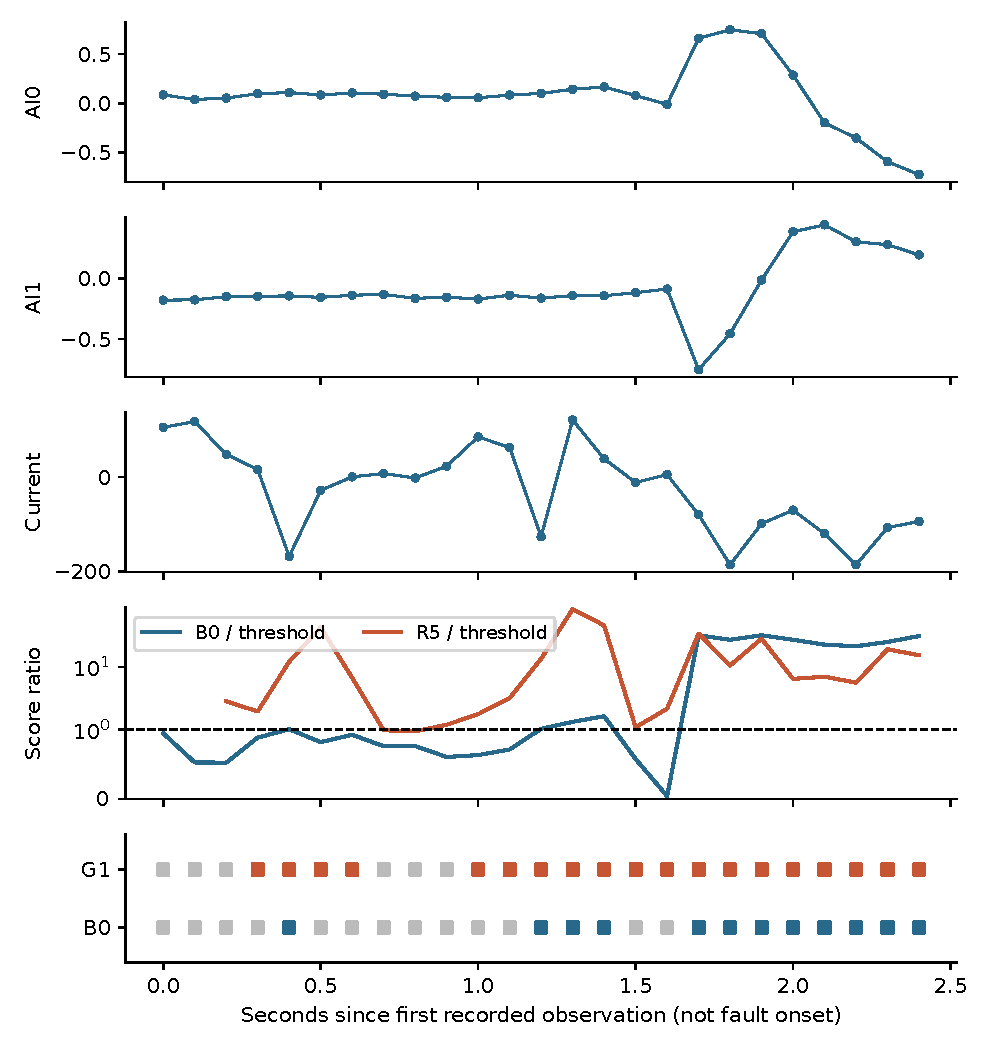
\includegraphics[width=.76\textwidth]{figures/case.pdf}\caption{추가 탐지가 있는 H 구간 중 시간순으로 가장 이른 구간 전체. 센서의 물리 단위는 미확인이다. 회색 사각형은 비경보, 색 사각형은 경보다. 현재 잔차는 현재 목표 관측 수신 뒤 계산되며 첫 경보 0.4초와 0.3초는 실제 고장 시작 기준이 아니다. 공백을 선으로 연결하지 않았다.}\label{fig:case}\end{figure}
\clearpage\begin{figure}[t]\centering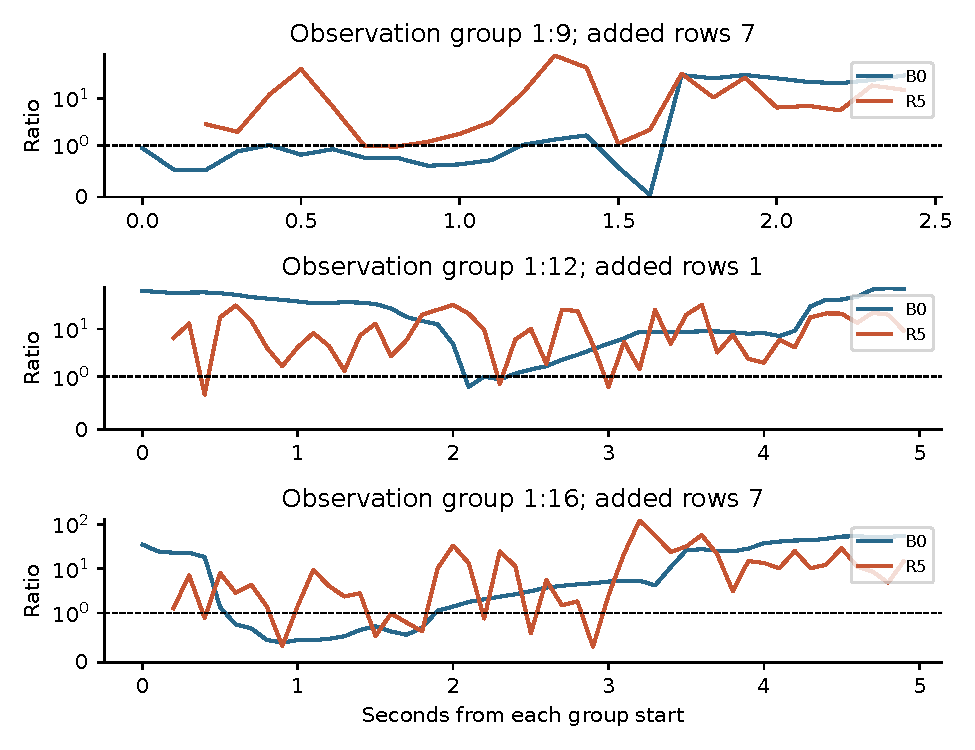
\includegraphics[width=.86\textwidth]{figures/all_affected.pdf}\caption{추가 탐지가 생긴 세 H 구간을 별도 축으로 표시했다. 구간 사이 관측 공백을 연결하지 않는다. 센서 패턴만으로 물리 고장 원인을 확정하지 않는다.}\end{figure}
\section{자료 사용 이력과 구현 검증의 단위}
\begin{figure}[h]\centering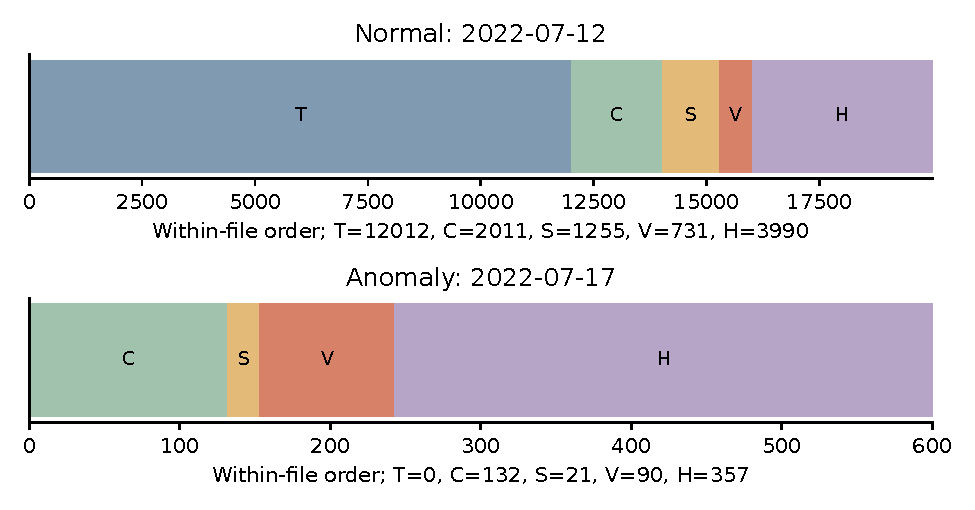
\includegraphics[width=.92\textwidth]{figures/roles.pdf}\caption{파일별 관측 순서와 역할. 날짜가 다르므로 두 축을 동시 관측으로 해석하지 않는다. C의 이상 132행은 과거 라벨 보정 용도이고 현재 G1 임계값에는 사용하지 않는다.}\end{figure}
행별 사용 감사는 고유 20,599행의 기존 사용을 모두 확인했다. 정상 중복 한 행은 이미 사용한 관측의 사본이다. 입력 창과 예측잔차의 과거 문맥도 사용으로 추적했다. 일부 개별 실험의 완전한 계보가 불명확하다는 사실은 그 행이 미사용이라는 뜻이 아니다. 별도 수집 신규 자료는 없으며 독립 새 자료 성능 검증은 미실시다.

감사 시점 기준 G1 개발·선정은 1회, 고정 검증은 1회, 전체 재현은 최소 2회다. 같은 S/V/H를 사용한 선행 개발 회차는 최소 4회다. 더 넓은 관련 이력의 PCA fit 절차 최소 106개는 후보 수가 아니며, 절차마다 spectrum과 유지 성분 PCA를 각각 적합하므로 fit 호출 수와도 단위가 다르다. R5 최소 5회에는 검증용 계수 재구성 2회가 포함된다. 구현 통과 항목 454건은 $151\times2+76\times2$의 반복 포함 합계이지 454개 후보나 독립 성능 시험이 아니다. 이번 원고 패키지의 추가 재현은 그 감사 마감 이후의 작업으로 별도 기록했다.

현재 해시는 파일 동일성의 근거이지 과거 사전 등록 시각의 독립 증명은 아니다. Git 저장소 이력은 없고 일부 같은 이름의 fit 로그는 덮어쓰여 전체 실행 횟수를 확정할 수 없다. 민감한 인증정보와 무관한 대화는 패키지에서 제외하고 필요한 연구 방향 변경과 완료 기록만 근거로 연결했다.

\begin{table}[!ht]\centering\caption{재현 검증의 범위. 성공한 구현 검사는 현장 성능의 독립 증거가 아니다.}\begin{tabularx}{\textwidth}{lX}\toprule
항목 & 근거와 범위\\\midrule
선정 모델 동일성 & B0/R5 원본 SHA-256, 모델 manifest, 실제 고정 임계값.\\
행·점수 정렬 & 동일 원행·라벨·판정, strict 경계와 수치 허용오차를 별도 기록.\\
인과적 동작 & 과거 미래값 변조 검사, 전체 원래 분할의 online/batch 비교, 보고용 경계에서 비초기화.\\
결측 입력 & 원 helper 문제를 보존하고 외부 wrapper가 거부; 실측 자료에는 결측 없음.\\
고정 학습 재현 & 정상 T에서 PCA 두 경로와 R5만 적합, 정상 C 보정, 선정 모델 비대체.\\
이식·문서 & 별도 해제 폴더 실행, 소스 PDF 빌드, CRC·해시·페이지 점검의 실제 기록.\\
독립 성능 & 별도 신규 수집 자료가 없어 미실시.\\\bottomrule\end{tabularx}\end{table}

\section{재현 패키지의 읽는 순서와 남은 자료}
START\_HERE\_ko.md에서 논문과 단점 중심 자체 검토 보고서, README의 실행 명령, evidence\_map.csv 순서로 읽을 수 있다. 원본 데이터와 중복 매핑, 고정 split, 정상 학습 입력·calibration 점수 재생성 코드, 모델 객체, 대조군 예측, 사건별 결과, 이전 후보 실패 기록을 포함한다. 원본부터 필요한 구성요소만 학습하는 경로와 저장 모델로 주요 결과를 재현하는 경로를 분리했다. 기존 전체 탐색을 기본 실행에서 반복하지 않는다.

미확인 물리 단위·장비·고장 시작·운전조건·독립 수집 자료와 완전한 과거 실행 이력은 새 코드로 대체할 수 없다. 저자·지원·이해상충 정보도 임의 작성하지 않았다. 데이터 이용조건이 불명확하므로 보관용 패키지를 공개 배포 허가나 자동 익명 보충자료로 취급하지 않는다. 동봉된 적대적 보고서는 최종 원고와 근거를 대조한 저자 측 AI 보조 검토이며 외부 심사 또는 실제 학회 판정이 아니다.
\end{document}
